\documentclass[12pt]{report}
\title{Predator Prey Model}
\author{Names Here}
\date{November 2011}

\usepackage{tikz}
\usepackage{verbatim} 
\usepackage{pict2e}
\usepackage[pdftex]{hyperref}

\begin{document}

\usetikzlibrary{shapes,arrows}


\tikzstyle{block} = [rectangle, draw, fill=blue!20, 
    text width=5em, text centered, rounded corners, minimum height=4em]
\tikzstyle{line} = [draw, -latex']

\maketitle

\begin{abstract}
\end{abstract}

\tableofcontents

\chapter{Introduction}

% i just wrote this to get the report started - feel free to change or add to it

In this task we worked as a group to implement a 2D, sequential predator-prey algorithm with spatial diffusion
in Java. We tried to design the program in such a way as to take advantage of Java's object-orientated, modular nature. 
Due to the large size of our group we also decided to develop a GUI for the program, although the code was designed 
in such a way as to be usable from the command line as well. -----is it?-----\newline{}

There is always some compromise between readability and performance in coding, and we tried to keep this balance in mind
when designing our code. We made best use of class structure whilst still keeping our implementation of the given 
algorithm as efficient as possible.\newline{}

The predator prey algorithm implemented in this project crudely models the interaction between population densities of different animals, specifically Hares and Pumas. Each population has a self-interaction coefficient (birth for Hares, death for Pumas) and a coefficient describing how it interacts with other species' populations. \newline{}

These populations exist on a `world' consisting of land and water, and are also able to diffuse across land squares with a rate determined by a diffusion coeffient. Thus, each population has N+1 coefficients which determine it's behaviour, where N is the number of animals.

\chapter{Model} %dmitry

$H_{ij}^{new}=H_{ij}^{old} + {\Delta}t(C_{1}H_{ij}^{old}+C_{2}H_{ij}^{old}P_{ij}^{old} + l(H_{i+1j}^{old} + H_{i-1j}^{old} + H_{ij+1}^{old} + H_{ij-1}^{old}-H_{ij}^{old}))$


\vspace{30 mm}

\noindent for k=1:NumberOfAnimals\newline{}
if (k=ThisAnimal) then\newline{}
$N_{k}^{new}=N_{k}^{old} + {\Delta}tC_{k}(k)N_{k}^{old}$\newline{}
else\newline{}
$N_{k}^{new}=N_{k}^{old} + {\Delta}tC_{k}(k)N_{k}^{old}N_{ThisAnimal}^{old}$\newline{}
end if\newline{}
end

where

\[ C_{Hare} = \left( \begin{array}{cc}
H & PH \end{array} \right)\] 

\chapter{Design \& Implementation}
   \section{Code}
      \subsection{Structure} %simon (dmitry to make flowchart)
      \subsection{Algorithm} %matt
      \subsection{Input/Output} %milena
      \subsection{GUI} %dmitry
   
   \section{Tools}
      \subsection{SVN} %matt
      \subsection{Makefile} %tom
      \subsection{Unit Testing} %jorge

\chapter{Performance Analysis}
   \section{Testing} %chen+tom
   \section{Analysis} %tom+chen
   
   % GNUPLOT: LaTeX picture with Postscript
\begingroup
  \makeatletter
  \providecommand\color[2][]{%
    \GenericError{(gnuplot) \space\space\space\@spaces}{%
      Package color not loaded in conjunction with
      terminal option `colourtext'%
    }{See the gnuplot documentation for explanation.%
    }{Either use 'blacktext' in gnuplot or load the package
      color.sty in LaTeX.}%
    \renewcommand\color[2][]{}%
  }%
  \providecommand\includegraphics[2][]{%
    \GenericError{(gnuplot) \space\space\space\@spaces}{%
      Package graphicx or graphics not loaded%
    }{See the gnuplot documentation for explanation.%
    }{The gnuplot epslatex terminal needs graphicx.sty or graphics.sty.}%
    \renewcommand\includegraphics[2][]{}%
  }%
  \providecommand\rotatebox[2]{#2}%
  \@ifundefined{ifGPcolor}{%
    \newif\ifGPcolor
    \GPcolortrue
  }{}%
  \@ifundefined{ifGPblacktext}{%
    \newif\ifGPblacktext
    \GPblacktexttrue
  }{}%
  % define a \g@addto@macro without @ in the name:
  \let\gplgaddtomacro\g@addto@macro
  % define empty templates for all commands taking text:
  \gdef\gplbacktext{}%
  \gdef\gplfronttext{}%
  \makeatother
  \ifGPblacktext
    % no textcolor at all
    \def\colorrgb#1{}%
    \def\colorgray#1{}%
  \else
    % gray or color?
    \ifGPcolor
      \def\colorrgb#1{\color[rgb]{#1}}%
      \def\colorgray#1{\color[gray]{#1}}%
      \expandafter\def\csname LTw\endcsname{\color{white}}%
      \expandafter\def\csname LTb\endcsname{\color{black}}%
      \expandafter\def\csname LTa\endcsname{\color{black}}%
      \expandafter\def\csname LT0\endcsname{\color[rgb]{1,0,0}}%
      \expandafter\def\csname LT1\endcsname{\color[rgb]{0,1,0}}%
      \expandafter\def\csname LT2\endcsname{\color[rgb]{0,0,1}}%
      \expandafter\def\csname LT3\endcsname{\color[rgb]{1,0,1}}%
      \expandafter\def\csname LT4\endcsname{\color[rgb]{0,1,1}}%
      \expandafter\def\csname LT5\endcsname{\color[rgb]{1,1,0}}%
      \expandafter\def\csname LT6\endcsname{\color[rgb]{0,0,0}}%
      \expandafter\def\csname LT7\endcsname{\color[rgb]{1,0.3,0}}%
      \expandafter\def\csname LT8\endcsname{\color[rgb]{0.5,0.5,0.5}}%
    \else
      % gray
      \def\colorrgb#1{\color{black}}%
      \def\colorgray#1{\color[gray]{#1}}%
      \expandafter\def\csname LTw\endcsname{\color{white}}%
      \expandafter\def\csname LTb\endcsname{\color{black}}%
      \expandafter\def\csname LTa\endcsname{\color{black}}%
      \expandafter\def\csname LT0\endcsname{\color{black}}%
      \expandafter\def\csname LT1\endcsname{\color{black}}%
      \expandafter\def\csname LT2\endcsname{\color{black}}%
      \expandafter\def\csname LT3\endcsname{\color{black}}%
      \expandafter\def\csname LT4\endcsname{\color{black}}%
      \expandafter\def\csname LT5\endcsname{\color{black}}%
      \expandafter\def\csname LT6\endcsname{\color{black}}%
      \expandafter\def\csname LT7\endcsname{\color{black}}%
      \expandafter\def\csname LT8\endcsname{\color{black}}%
    \fi
  \fi
  \setlength{\unitlength}{0.0500bp}%
  \begin{picture}(7200.00,4536.00)%
    \gplgaddtomacro\gplbacktext{%
      \csname LTb\endcsname%
      \put(1100,640){\makebox(0,0)[r]{\strut{}-3.5}}%
      \put(1100,1111){\makebox(0,0)[r]{\strut{}-3.0}}%
      \put(1100,1582){\makebox(0,0)[r]{\strut{}-2.5}}%
      \put(1100,2053){\makebox(0,0)[r]{\strut{}-2.0}}%
      \put(1100,2523){\makebox(0,0)[r]{\strut{}-1.5}}%
      \put(1100,2994){\makebox(0,0)[r]{\strut{}-1.0}}%
      \put(1100,3465){\makebox(0,0)[r]{\strut{}-0.5}}%
      \put(1100,3936){\makebox(0,0)[r]{\strut{} 0.0}}%
      \put(1220,440){\makebox(0,0){\strut{} 0}}%
      \put(2167,440){\makebox(0,0){\strut{} 1}}%
      \put(3113,440){\makebox(0,0){\strut{} 2}}%
      \put(4060,440){\makebox(0,0){\strut{} 3}}%
      \put(5007,440){\makebox(0,0){\strut{} 4}}%
      \put(5953,440){\makebox(0,0){\strut{} 5}}%
      \put(6900,440){\makebox(0,0){\strut{} 6}}%
      \put(400,2288){\rotatebox{90}{\makebox(0,0){\strut{}log$_{10}$ Time/Cell [s]}}}%
      \put(4060,140){\makebox(0,0){\strut{}log$_{10}$ Number of Cells}}%
      \put(4060,4236){\makebox(0,0){\strut{}Run Time/Number of Cells vs. Number of Cells}}%
    }%
    \gplgaddtomacro\gplfronttext{%
      \csname LTb\endcsname%
      \put(5997,3773){\makebox(0,0)[r]{\strut{}Run Time/Number of Cells}}%
    }%
    \gplbacktext
    \put(0,0){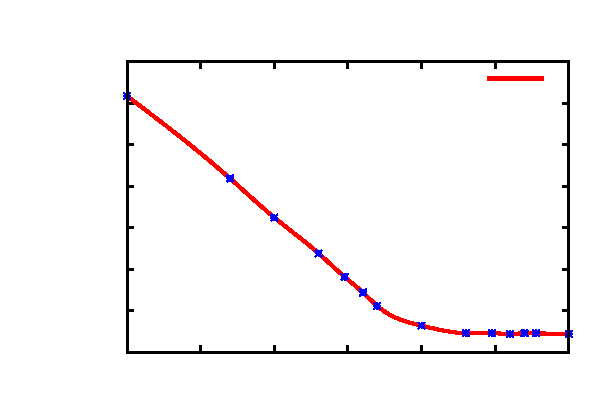
\includegraphics{figs/overhead}}%
    \gplfronttext
  \end{picture}%
\endgroup


\chapter{Conclusions} %everyone

\chapter{Group Evaluation} %everyone

\end{document}